% 高斯消元法程序

\pentry{线性方程组高斯消元法\upref{GAUSS}}

这里给出一个简单的程序演示高斯消元法的基本步骤. 注意在实际应用中, 我们解线性方程组一般使用 Matlab 的反斜杠算符:\x{x=A\textbackslash y} ,其中 $\mat A$ 是系数矩阵,$\vec y$ 是常数列,$\vec x$ 是未知量。

\Code{GaussEli}

与“高斯消元法\upref{GAUSS}” 中的步骤略有不同的是, 该程序在处理每一行 \x{A(ii,:)}  时都会试图做一个行交换使系数 \x{A(ii,q(ii))} 的绝对值尽可能大。 这是为了减小数值误差: 试想如果 \x{A(ii,q(ii))} 的解析值为 0, 但由于数值误差, 计算出来是一个很小的数(例如 \x{1e-15}), 那么用其消元时就可能需要将第 \x{ii} 行乘以一个很大的系数(例如 \x{1e15})再加到另一行上, 导致程序不稳定。

用\autoref{GAUSS_ex2}\upref{GAUSS} 中的增广矩阵测试程序如下:

\begin{Command}
>> A = [1 1 -1 1; 2 2 -2 1; 1 1 0 2; 2 2 -1 5]\\
>> y = [3; 7; 3; 4];\\
>> [A, q] =GaussEli([A,y],true)
\end{Command}

运行结果为(程序的中间输出略)
\begin{figure}[ht]
\centering
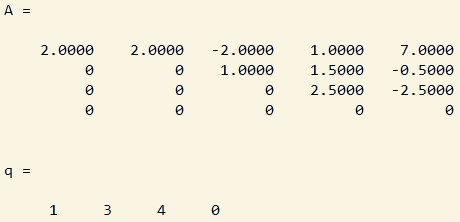
\includegraphics[width=10cm]{./figures/GauEli1.png}
\caption{运行结果} \label{GauEli_fig1}
\end{figure}
